\documentclass{article} 
\usepackage{iclr2026_conference,times}
\usepackage{macros}
\usepackage{hyperref}
\usepackage{url}
\usepackage[toc,page,header]{appendix}
\usepackage{geometry}

\geometry{margin=1in}

\usepackage{minitoc}

\renewcommand \thepart{}
\renewcommand \partname{}

\title{ARPE Title}

\author{}

\newcommand{\greg}[1]{{\color{indigo}[Gregoire]: #1}}
\newcommand{\fel}[1]{{\color{gold}[Fel]: #1}}
\newcommand{\agus}[1]{{\color{green}[Agus]: #1}}
\newcommand{\boutin}[1]{{\color{pink}[Baltringueur]: #1}}
\newcommand{\thomas}[1]{{\color{blue}[Thomas]: #1}}

\widowpenalty=10000
\clubpenalty=10000


\begin{document}

\doparttoc % Tell to minitoc to generate a toc for the parts
\faketableofcontents % Run a fake tableofcontents command for the partocs

\maketitle

\begin{abstract}
...
\end{abstract}

% ====================================================================================================
\part{Neural Circuits as a Design Principle} % serves as introduction, laying the groundwork and motivation for the rest of the report.
% ====================================================================================================

% TODO : add to the example section sec:neural_circuits that the model could be further improved by including potential higher order derivatives or time delays.

\greg{This part serves as introduction, biblio, background etc. for the rest of the document.}

\greg{Add note on magno and parvo pathways (in vision) as an example of parallel pathways with different dynamics and functions. Magno is fast and feedback connection typically target magno pathways to meet up with slower parvo feedforward and recurrent pathways at a target area, implementing predictive and modulatory processing. Also, FB is typically long ranged (spatially) while recurrent is local - spectral vs spatial parameterisation of orthogonal convolution. We can model magno as skip connections, in which case the overall pathway reduces to a simple recurrence, and SSM solve both recurrent and feedback connection for the price of none (!). If we want to clearly separate FB and REC, we can use two layers, one parameterised spectrally, one spatially. This would cost a bit more but would be more biologically plausible and more interpretable.}

% ----------------------------------------------------------------------------------------------------
\section{Introduction}
% ----------------------------------------------------------------------------------------------------

\paragraph{} Present the overall project, motivations, initial goals, how it fits into my program, etc. Present the structure of the report.

% ----------------------------------------------------------------------------------------------------
\section{Biological and Computational Motivation}
% ----------------------------------------------------------------------------------------------------

\paragraph{}Brief overview of computational neuroscience, biological neural circuits and modeling efforts, and links to machine learning history.

% ----------------------------------------------------------------------------------------------------
\section{Formalizing Neural Circuits}
% ----------------------------------------------------------------------------------------------------
\label{sec:neural_circuits}

\input{sections/part_intro/neural_circuit.tex}

% ----------------------------------------------------------------------------------------------------
\section{Neural Circuits in Brain Sciences}
% ----------------------------------------------------------------------------------------------------
\label{sec:neural_circuits_brain_science}

\input{sections/part_intro/neural_circuits_brain_science.tex}

% ----------------------------------------------------------------------------------------------------
\section{Neural Circuits in Machine Learning}
% ----------------------------------------------------------------------------------------------------

\paragraph{}Overview of existing machine learning architectures that can be interpreted as neural circuits, highlighting their structure and function. State how most are purely feedforward, with recurrent architectures still marginal despite the recent SSM developpements, and feedback connections being even more rare and constrained to specific use cases such as predictive coding. Transformers can have a sort of time "recurrence" through positional encoding, but this isn't fit for long range sequences due to computational complexity. Plus, recurrence is quite artificial as it is added through attention masks and positional encoding, there is no hidden state that evolves over time. Each token is independent from the others, and it works thanks to full memory preservation. Recurrent and feedback architectures are not only more biologically plausible, but they also offer potential advantages in terms of efficiency, adaptability, interpretability and dynamics depending on the task.

% ----------------------------------------------------------------------------------------------------
\section{Scope and Research Questions}
% ----------------------------------------------------------------------------------------------------

\paragraph{}We explore several aspects that naturally emerge from the above framework. First is architecture design grounded in neural circuits for a single modality (here, vision) (part II). Second, is the integration of unimodal circuits into a single multimodal one (part III and IV). Finally, in part V we explore the possibility of a universal neural circuit, akin to universal turing machines, that could simulate any other neural circuit, possibly under some constraints to make the problem tractable. This could serve as a foundation for a foundation model for brain science.

% ====================================================================================================
\part{Constructing Better Vision Circuits} % main technical contribution, proposing ConvSSM as a new architecture for vision tasks, inspired by neural circuits.
% ====================================================================================================

\section*{Part Outline}

\paragraph{}In this part, we explore how the circuit formalism of part I can guide the design of new architectures. Specifically, our goal is to introduce horizontal recurrent connections, where current SSMs only have self-recurrence.

% ----------------------------------------------------------------------------------------------------
\section{Related Work}
% ----------------------------------------------------------------------------------------------------

\paragraph{}ConvNet, SSM, ConvS4, hGRU, etc. Also, dino is approximated by a recurrent architecture with just two layers (Fel et al).

% ----------------------------------------------------------------------------------------------------
\section{ConvSSM Definition}
% ----------------------------------------------------------------------------------------------------
\label{sec:ConvSSM_definition}


\paragraph{State Space Model.} The state space model (SSM) is a class of recurrent model with linear recurrent dynamics. Their most general formulation is that of continuous-time (\Cref{eq:ssm}), which can be discretised as in \Cref{eq:ssm:recurrence}, with transition matrices depending on the desired step size following \Cref{eq:zoh}. Parameterizing transition matrices of the continuous time formulation allows to handle arbitrary sampling rates for free. Additionally, Mamba \citep{TODO:Mamba} takes advantage of this continuous time formulation and discretization step to derive a data-adaptive gating mechanism to give more or less importance to the present input.

\begin{minipage}[t]{.30\linewidth}
  \begin{subequations}
    \label{eq:ssm}
    \begin{align}
      h'(t) &= A h(t) + B x(t) \\
      y(t) &= C h(t)
    \end{align}
  \end{subequations}
\end{minipage}%
\begin{minipage}[t]{.30\linewidth}
  \begin{subequations}
    \label{eq:ssm:recurrence}
    \begin{align}
    \label{eq:ssm:recurrence:1}
      h_{t} &= \overline{A} h_{t-1} + \overline{B} x_t \\
    \label{eq:ssm:recurrence:2}
      y_t &= C h_t
    \end{align}
  \end{subequations}
\end{minipage}%
\begin{minipage}[t]{.39\linewidth}
  \begin{subequations}%
    \label{eq:ssm:convolution}
    \begin{align}
      \label{eq:ssm:convolution:1}
      \bm{\overline{K}} &= (\bm{C}\bm{\overline{B}}, \bm{C}\bm{\overline{A}}\bm{\overline{B}}, \dots, \bm{C}\bm{\overline{A}}^{k}\bm{\overline{B}}, \dots) \\
      \label{eq:ssm:convolution:2}
      y &= x \ast \bm{\overline{K}}
    \end{align}
  \end{subequations}
\end{minipage}

\paragraph{Discretisation.} Various rules can be used for discretisation, such as the zero-order hold (ZOH) whose solution is given in \Cref{eq:zoh}.
\begin{equation}
\label{eq:zoh}
\overline{A} = e^{\Delta \bm{A}}
\qquad
\overline{B} = (\Delta \bm{A})^{-1} (e^{\Delta \bm{A}} - \bm{I}) \cdot \Delta \bm{B}
\end{equation}
where $\Delta$ is the time step.

\paragraph{Spatial Coupling.} Rewriting \Cref{eq:ssm} to include horizontal connections yields \Cref{eq:conv_ssm_continuous}, with the corresponding discrete time formulations in \Cref{eq:conv_ssm_discrete}.

\begin{minipage}[t]{.45\linewidth}
  \begin{subequations}
    \label{eq:conv_ssm_continuous}
    \begin{align}
    \label{eq:conv_ssm_continuous:1}
      \frac{\partial h}{\partial t}(r,t) &= K_h \ast h(r, t) + K_x \ast x(r, t) \\
      y(r, t) &= K_y \ast h(r, t)
    \end{align}
  \end{subequations}
\end{minipage}%
\begin{minipage}[t]{.45\linewidth}
  \begin{subequations}
    \label{eq:conv_ssm_discrete}
    \begin{align}
    \label{eq:conv_ssm_discrete:1}
      h_{t} &= \overline{K}_h \ast h_{t-1} + \overline{K}_x \ast x_t \\
    \label{eq:conv_ssm_discrete:2}
      y_t &= K_y \ast h_t
    \end{align}
  \end{subequations}
\end{minipage}

However, discretization of the convolution kernel isn't as straightforward due to spatial coupling. Indeed, in order to be in the linear recurrence case, we need to view a whole image as a single vector $x\in \R^{(h\cdot w) \times c}$ and expand the convolution kernel into a circulant matrix $A \in \R^{(h\cdot w)^2 \times c^2}$. Now, following \Cref{eq:zoh}, we can compute $\overline{A}$. However, $\overline{B}$ requires the inverse of $A$ which typically has full spatial support, making it intractable in spatial domain.

By diagonalizing the circulant matrix in spectral domain, the set of spatially coupled partial differential equations (PDE) from \Cref{eq:conv_ssm_continuous:1} becomes a set of spectrally decoupled ordinary differential equations (ODE) (\Cref{eq:conv_ssm_continuous_spectral})~:

\begin{minipage}[t]{.45\linewidth}
  \begin{subequations}
    \begin{align}
    \label{eq:conv_ssm_continuous_spectral}
      \frac{\partial \widehat{h}}{\partial t}(w,t) &= \widehat{K}_h(w) \widehat{h}(w, t) + \widehat{K}_x(w) \widehat{x}(w, t)
    \end{align}
  \end{subequations}
\end{minipage}%

making \Cref{eq:zoh} applicable to every spatial frequency separately~:
\begin{equation}
\label{eq:zoh_spectral}
\overline{K}_h(w) = e^{\Delta \bm{\widehat{K}}_h(w)}
\qquad
\overline{K_x}(w) = (\Delta \bm{\widehat{K}}_h(w))^{-1} (e^{\Delta \bm{\widehat{K}}_h(w)} - \bm{I}) \cdot \Delta \bm{\widehat{K}}_x(w)
\end{equation}

\paragraph{Stability.} The continuous time ODEs imply exponential dynamics of the state over time. This dynamics are controlled by the eigenvalues $\lambda^A_i$ of the transition matrix $A$ ($\widehat{K}_h(w)$ in our case). The imaginary part controls the angular speed, while the real part controls the modulus' exponential growth. Thus, stability is achieved when

\begin{align}
    \label{eq:stability}
    \mathrm{Re}(\lambda^A_i) \leq 0
\end{align}

The corresponding discrete time condition is thus given by
\begin{align}
    \label{eq:discrete_stability}
    |\lambda^{\overline{A}}_i| \leq 1
\end{align}

State of the art SSM parameterisation enforces \Cref{eq:discrete_stability} on $A$. They remark that in general it does not seem to work (which is expected as it is not the correct condition), but in the special case of HiPPO matrices, it happens to work well. Through a happy accident, these matrices can be decomposed in a normal plus low rank (NPLR) form with a normal component that satisfies the correct condition of \Cref{eq:stability}.

\paragraph{Link to Neural Circuits.} As mentioned in \cref{sec:background}, the state space model implements \emph{recurrent} connections through linear dynamics to make them parallelisable. State of the art approaches in vision make these \emph{self-recurrent} only \citep{TODO}. Our approach adds \emph{intra-recurrence} through \emph{horizontal} connections for visual systems in such a way that preserves computational stability and complexity, while adding expressivity and biological plausibility.


% ----------------------------------------------------------------------------------------------------
\section{ConvSSM Complexity}
% ----------------------------------------------------------------------------------------------------
\label{sec:ConvSSM_complexity}


Recall that the goal is to implement the following recurrence :
\begin{align}
\label{eq:convssm_recurrence}
    h_{t+1}=\overline{K}_h{\mathrm{A}} \ast h_t + \overline{K}_x{\mathrm{B}}\ast I_{t+1}
\end{align}
where $h_i$ is the hidden state at time step $i$, $I_i$ is the input image - or feature map. $\overline{K}_h{\mathrm{A}}$ and $\overline{K}_xK_{\mathrm{B}}$ are convolution kernels. For simplicity, we will omit $\overline{K}_xK_{\mathrm{B}}$ in the remainder of this section. We show that computing the sequence of hidden states $(h_i)_{i\in\intint{0}{T-1}}$ given a sequence of inputs $(I_i)_{i\in\intint{0}{T-1}}$ can be seen as computing a scan operation.

We analyse the complexity of the parallel scan algorithm to show why convolutions in spatial domain make the complexity explode, and how doing convolutions in spectral domain preserves $O(\log T)$ complexity. We consider both the work complexity $W$, measuring the total amount of atomic operations to perform, and the time complexity under unlimited parallelization $T_\infty$, measuring the longest sequence of atomic operations remaining after optimal parallelization.

We begin by addressing the main issue of the complexity explosion of convolutional SSMs in \cref{sec:scan_algo,sec:scan_SSM,sec:spatial_ConvSSM,sec:spectral_ConvSSM}. Our main result is \Cref{prop:spectral_conv_complexity}, where we show that we can achieve the same work and time complexity as a regular linear SSM. We then tackle the question of reducing the constant to make it tractable, using standard tricks, adapted to our framework, in \cref{sec:the_constant}.

\paragraph{Mamba-style note.} In this section, we consider transition matrices and transition kernels to be fixed over time. Note that it is entirely possible to have different weights at each time step simply by modifying the initial sequence of $(a_i)_{i\in I}$ defined below. In particular, following \citet{TODO:Mamba} one could parameterize $\Delta$ to depend on the present input $x_i$.

\subsection{The parallel scan algorithm}
\label{sec:scan_algo}

We first describe the parallel scan operation in the most general way. This operation is the core of the SSM parallelization. Let $(a_i)_{i\in I}\in M^I$ be elements of a monoid $(M,+,0)$, with $I=\intint{0}{T\!-\!1}$. The parallel scan is an algorithm that computes $(s_i=\sum_{j=0}^ia_j)_i\in I$. This algorithm is parallelisable and requires associativity of the $+$ operator and a neutral element $0$, hence the minimal requirement of a monoid structure. It proceeds in two sweeps mirroring each other. The first sweep proceeds in a tree like structure, with level $l$ of the tree computing $a^{l+1}_{k}\coloneqq a^l_{2k} + a^l_{2k+1}$, and initialised with $a^0_k\coloneqq a_k$. Once this upward sweep is over, the downward sweep computes mirror operations, with $b^0_1\coloneqq 0$ and $(b^{l+1}_{2k}, b^{l+1}_{2k+1}) = (b^{l}_{k}, b^{l}_{k} + a^{\log_2(T)-(l+1)}_{2k})$. The order is crucial here as $+$ is not required to be commutative. It is only required to be associative. In our application for SSM, it will not be commutative. We denote the parallel scan procedure as $\mathrm{Scan}((a_i)_{i\in I})$ or $\mathrm{Scan}$ for short.
\Cref{fig:parallel_scan_general} provides a visualisation of the entire procedure.

\begin{figure}[ht]
    \centering
    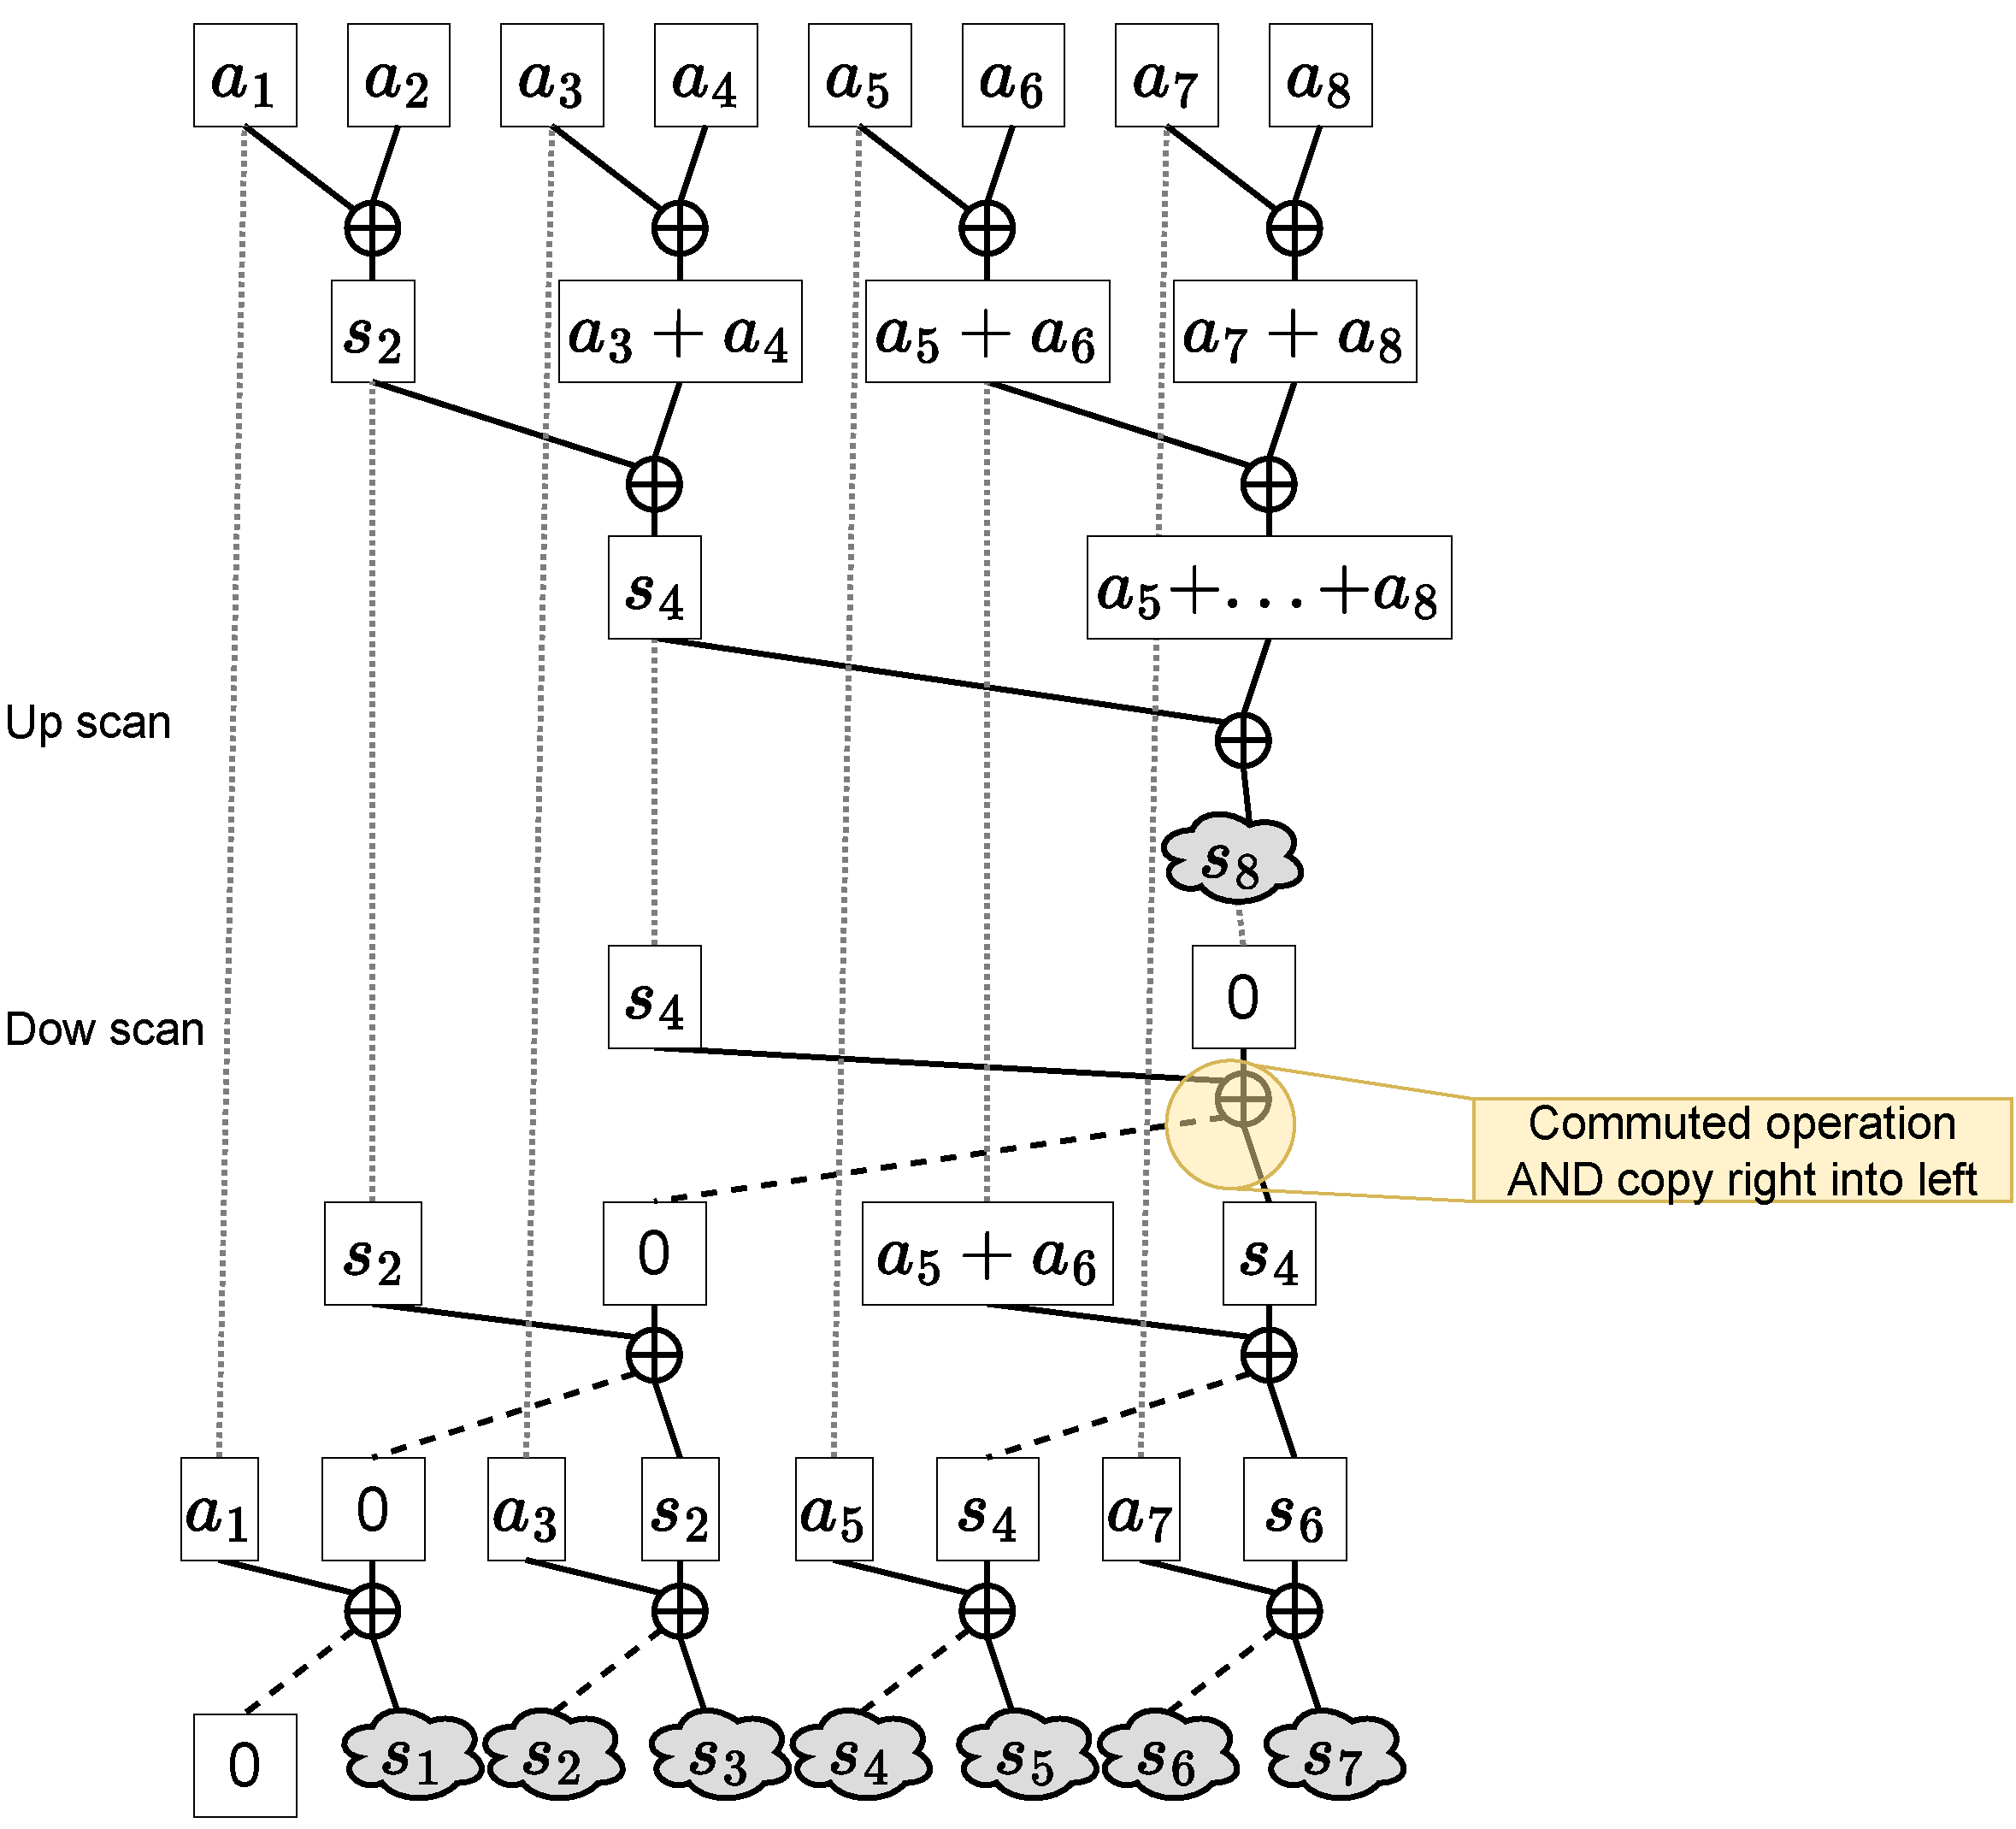
\includegraphics[height=0.3\textheight]{figures/scan_monoid.pdf}
    \hspace{20mm}
    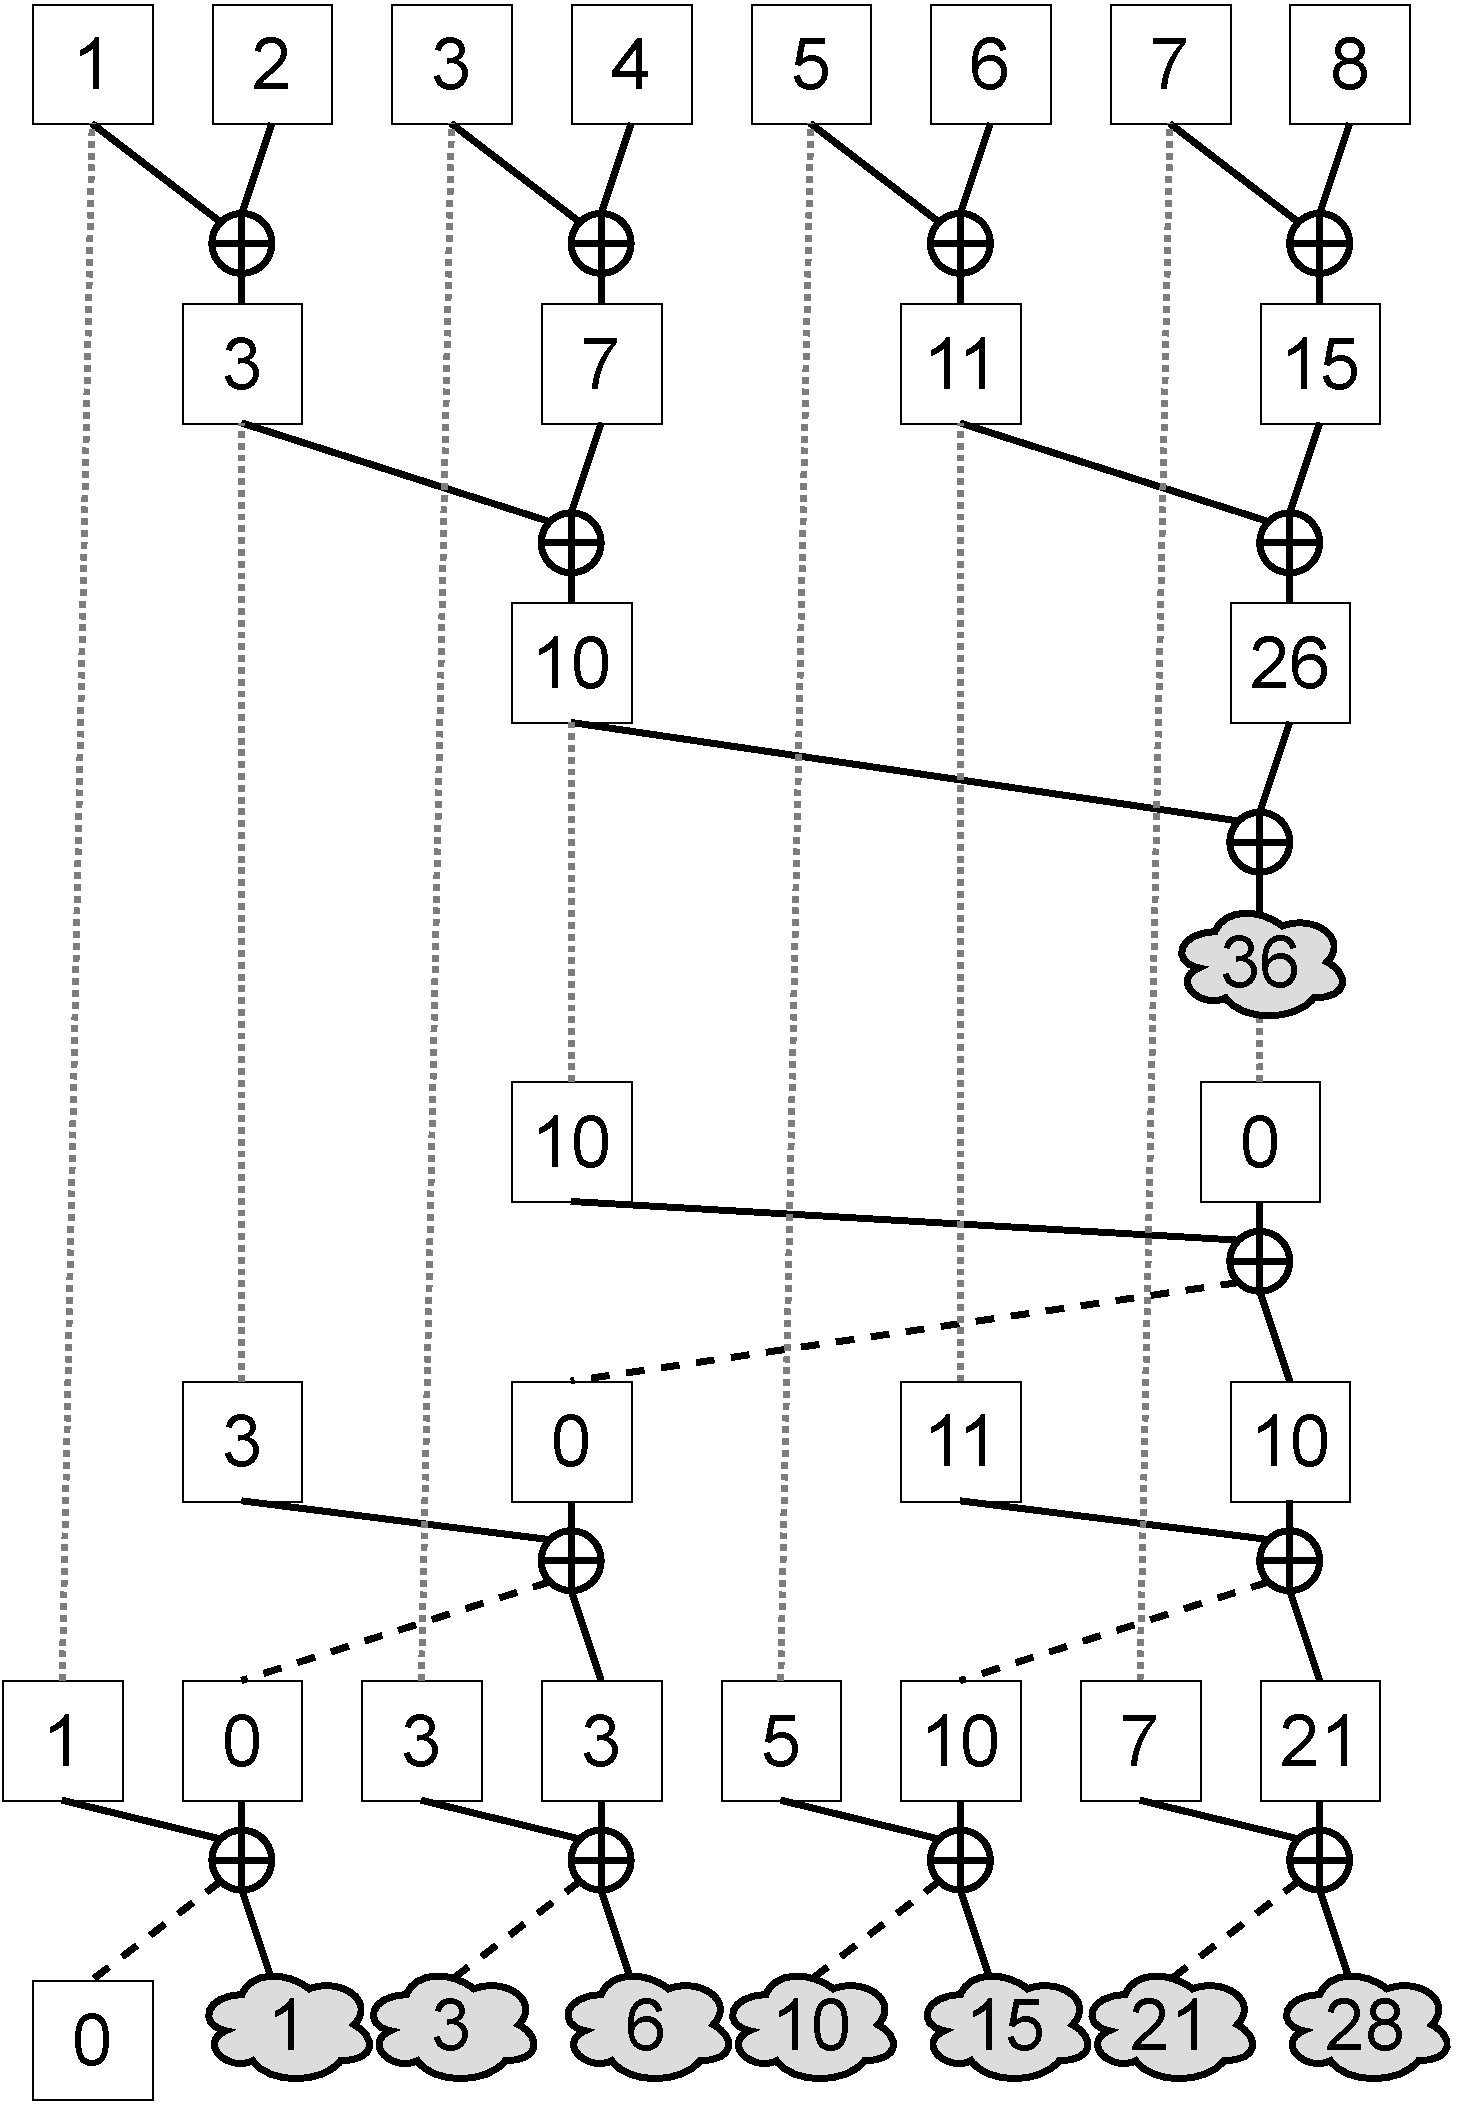
\includegraphics[height=0.3\textheight]{figures/scan_integer.pdf}
    \caption{\textbf{Left:} parallel scan with a generic monoid. \textbf{Right:} illustration on the spetial case of natural integers.}
    \label{fig:parallel_scan_general}
\end{figure}

The procedure described above yields $(\sum_{j=0}^{i-1}a_j)_{i\in I}$, with the cumulative sum being $a^{\log_2(T)}_{0}$ the intermediate result of the upward sweep. We analyse the work complexity $W$ and the time complexity $T_\infty$ of $\mathrm{Scan}$ in terms of floating point operations, where $W$ counts the total number of operations needed and $T_\infty$ counts the time complexity under unlimited parallelism.

\begin{proposition}[Parallel Scan Complexity for $(\N, +)$]
\label{prop:scan_integer_complexity}
    Let $(M, +) \coloneqq (\N, +)$ be the monoid of natural integers equipped with addition. Let $(a_i)_{i\in I}\in \N^I$ be a sequence of integers.

\begin{align}
    W(\mathrm{Scan})&= 2(T-1)\\
    T_\infty(\mathrm{Scan})&= 2\log_2 T
\end{align}
\end{proposition}

\begin{proof}
At level $l$ of the upward scan, $U_l = T/(2^{l+1})$ "$+$" operations are performed, each of them having a complexity of $1$. There are $\log_2 T$ levels in total. The same goes on for the downward scan, with $D_l = T/(2^{\log_2(T) - l})=2^{l}$ operations at level $l$. Therefore, the work complexity of level $l$ is $U_l$ (resp. $D_l$) while its time complexity is $1$ with unlimited parallelism. It follows that

\begin{align}
\label{eq:W_integer}
W &= 2\sum_{l=0}^{\log_2(T)-1}2^l=2(T-1)\\
\label{eq:T_integer}
T_\infty&= 2\sum_{l=0}^{\log_2(T)-1}1=2\log_2T
\end{align}
\end{proof}

\subsection{The case of SSM}
\label{sec:scan_SSM}

The case of SSMs is a little more complicated than that of real numbers. In SSMs, the recurrence is defined by \Cref{eq:convssm_recurrence} with the slight modification that kernel convolution is now matrix multiplication and taking $B = I$. Thus, the goal is to compute in parallel the hidden states $(h_i = \sum_{j=0}^i\overline{A}^{i-j}x_j)_i\in I$, where $x_i$ are vectors of dimension $d$ and $\overline{A}$ is a square matrix. This is almost but not quite what we need for the parallel scan. We define the following monoid:
\begin{align}
\label{eq:M_SSM}
    &M^{\mathrm{SSM}}\coloneqq \left\{a = (A, x)\mid A\!\in\!\mathcal{M}_{d}(\R),~x\!\in\!\R^d\right\}\\
\label{eq:+_SSM}
    &(A_a, x_a) +^{\mathrm{SSM}} (A_b,x_b)\coloneqq (A_b \odot A_a, A_b \cdot x_a + x_b)\\
\label{eq:0_SSM}
    &0^{\mathrm{SSM}}\coloneqq(I_d, 0)
\end{align}

With this monoid structure, and the sequence $(a_i)_{i\in I} \coloneqq ((A, x_i))_{i\in I} \in M^I$, the result of the parallel scan is $((A^i, \sum_{j=0}^iA^{i-j}x_j))_{i\in I}$. The complexity of the scan is less straightforward, but the complexity of each $+^{\mathrm{SSM}}$ operation depends only on $d$, it is a constant of $T$, and therefore, the overall time complexity of the scan is $T_\infty= O(\log T)$ and $W=O(T)$.

\begin{proposition}[SSM Complexity]
\label{prop:SSM_complexity}
    Let $(M, +) \coloneqq (M^{\mathrm{SSM}}, +^{\mathrm{SSM}})$ be the monoid defined by \Cref{eq:M_SSM,eq:+_SSM,eq:0_SSM}. Let $(a_i)_{i\in I}\in (M^{\mathrm{SSM}})^I$.

\begin{align}
    W(\mathrm{Scan})&= 2(T-1)(d^3+d^2+d)\\
    T_\infty(\mathrm{Scan})&= 2\log_2 (T) (d^3+d^2+d)
\end{align}
\end{proposition}

\begin{proof}
The proof of \Cref{prop:scan_integer_complexity} applies with the only difference that now, each $+^{\mathrm{SSM}}$ operation has complexity $d^3$ for the matrix multiplication on the left, $d^2$ for the matrix-vector multiplication and $d$ for the vector addition on the right.
\end{proof}

\subsection{The problem of convolution}
\label{sec:spatial_ConvSSM}

Moving from $d$ dimensional vectors to images with $c$ channels and $h \times w$ spatial dimension and from matrix multiplication to spatial convolution, we can rewrite our monoid structure as :
\begin{align}
    &M^{\mathrm{Conv}_1}\coloneqq \left\{a = (K, I)\mid \exists k_1, k_2,\quad K\!\in\!\R^{k_1\times k_2\times c\times c},~I\!\in\!\R^{h \times w \times c}\right\}\\
    &(K_a, I_a) +^{\mathrm{Conv}_1} (K_b,I_b)\coloneqq (K_b \circledast K_a, K_b \ast I_a + I_b)\\
    &0\coloneqq(I, 0)
\end{align}
\noindent where $\circledast$ is the convolution between two kernels and $\ast$ is the convolution between a kernel and an image:

\begin{align*}
    & \forall \left\{
\begin{aligned}
    &x\!\in\!\intint{0}{h\!-\!1}\\
    &y\!\in\!\intint{0}{w\!-\!1}\\
    &c_{\mathrm{out}}\!\in\!\intint{1}{c}
\end{aligned}
\right., (K\!\ast\!I)_{x,y,c_{\mathrm{out}}} = \sum_{u=0}^{k_1-1}\sum_{v=0}^{k_2-1}\sum_{i=1}^{c} K_{u,v,i,c_{\mathrm{out}}} I_{(x-u,y-v)\%(h,w),i}\\
    & \forall \left\{
\begin{aligned}
    &u\!\in\!\intint{0}{k_1\!+\!l_1\!-\!2}\\
    &v\!\in\!\intint{0}{k_2\!+\!l_2\!-\!2}\\
    &c_{\mathrm{in}},c_{\mathrm{out}}\!\in\!\intint{1}{c}
\end{aligned}
\right., (L \circledast K)_{u,v,c_{\mathrm{in}},c_{\mathrm{out}}} = \sum_{p=0}^{l_1-1}\sum_{q=0}^{l_2-1}\sum_{c_{k}=1}^{c} L_{p,q,c_{k},c_{\mathrm{out}}} K_{u-p,v-q,c_{\mathrm{in}},c_{k}}\text{, $K$ being zero-padded}
\end{align*}
\noindent with $L\!\in\!\R^{l_1\times l_2\times c \times c}$, $K\!\in\!\R^{k_1\times k_2\times c \times c}$ and $I\!\in\!\R^{h \times w \times c}$

With this structure, the key aspect is that the spatial size of the kernel resulting from $\circledast$ is the sum of the sizes of the input kernels. Therefore, the parallel scan algorithm operates on larger and larger kernel sizes, with sizes growing exponentially with the depth in the tree structure. The complexity of our $+$ operator is thus no more constant as it depends on the depth. The bottleneck is at the very last layer of the upward scan, where kernel size is $O(Tk)$, with $k$ the size of the original kernel $K$, resulting in a single $\ast$ operation whose complexity is in $O(T^2)$. This bottleneck is illustrated in \Cref{fig:parallel_scan_conv_spatial}.

\begin{proposition}[Spatial ConvSSM Complexity]
    Let $(M, +) \coloneqq (M^{\mathrm{Conv}_1}, +^{\mathrm{Conv}_1})$ be the monoid defined by \Cref{eq:M_SSM,eq:+_SSM,eq:0_SSM}. Let $(a_i)_{i\in I}\in (M^{\mathrm{Conv}_1})^I$.

\begin{align}
    W&= O(T^2)\\
    T_\infty&= O(W)
\end{align}
\end{proposition}

\begin{proof}
The proof of \Cref{prop:scan_integer_complexity} applies with the major difference that on the upward scan, at level $l$, each $+^{\mathrm{Conv}_1}$ operation has complexity $(k+(2^l-1)(k-1))\times (k+(2^l-1)(k-1))\times c^3 = O((2^l)^2\times k^2 \times c^3)$ for the kernel-kernel convolution on the left, $O(h \times w \times (2^l)^2\times k^2 \times c^2)$ for the kernel-image convolution and $h \times w\times c$ for the image addition on the right. The same goes on for the downward scan.

Thus, \Cref{eq:W_integer,eq:T_integer} become :

\begin{align}
\label{eq:W_conv}
W &= O(2 \sum_{l=0}^{\log_2(T)-1} 2^{\log_2(T)-(l+1)} \times \left[ (2^l)^2\times k^2 \times c^3 + h \times w \times (2^l)^2\times k^2 \times c^2\right])\\
&= O(T^2 \times k^2 \times c^3) + O(T^2 \times h \times w \times k^2 \times c^2)\\
\label{eq:T_conv}
T_\infty&= O(2\sum_{l=0}^{\log_2(T)-1} \left[ (2^l)^2\times k^2 \times c^3 + h \times w \times (2^l)^2\times k^2 \times c^2\right])\\
&= O(W)
\end{align}
\end{proof}

\begin{figure}[ht]
    \centering
    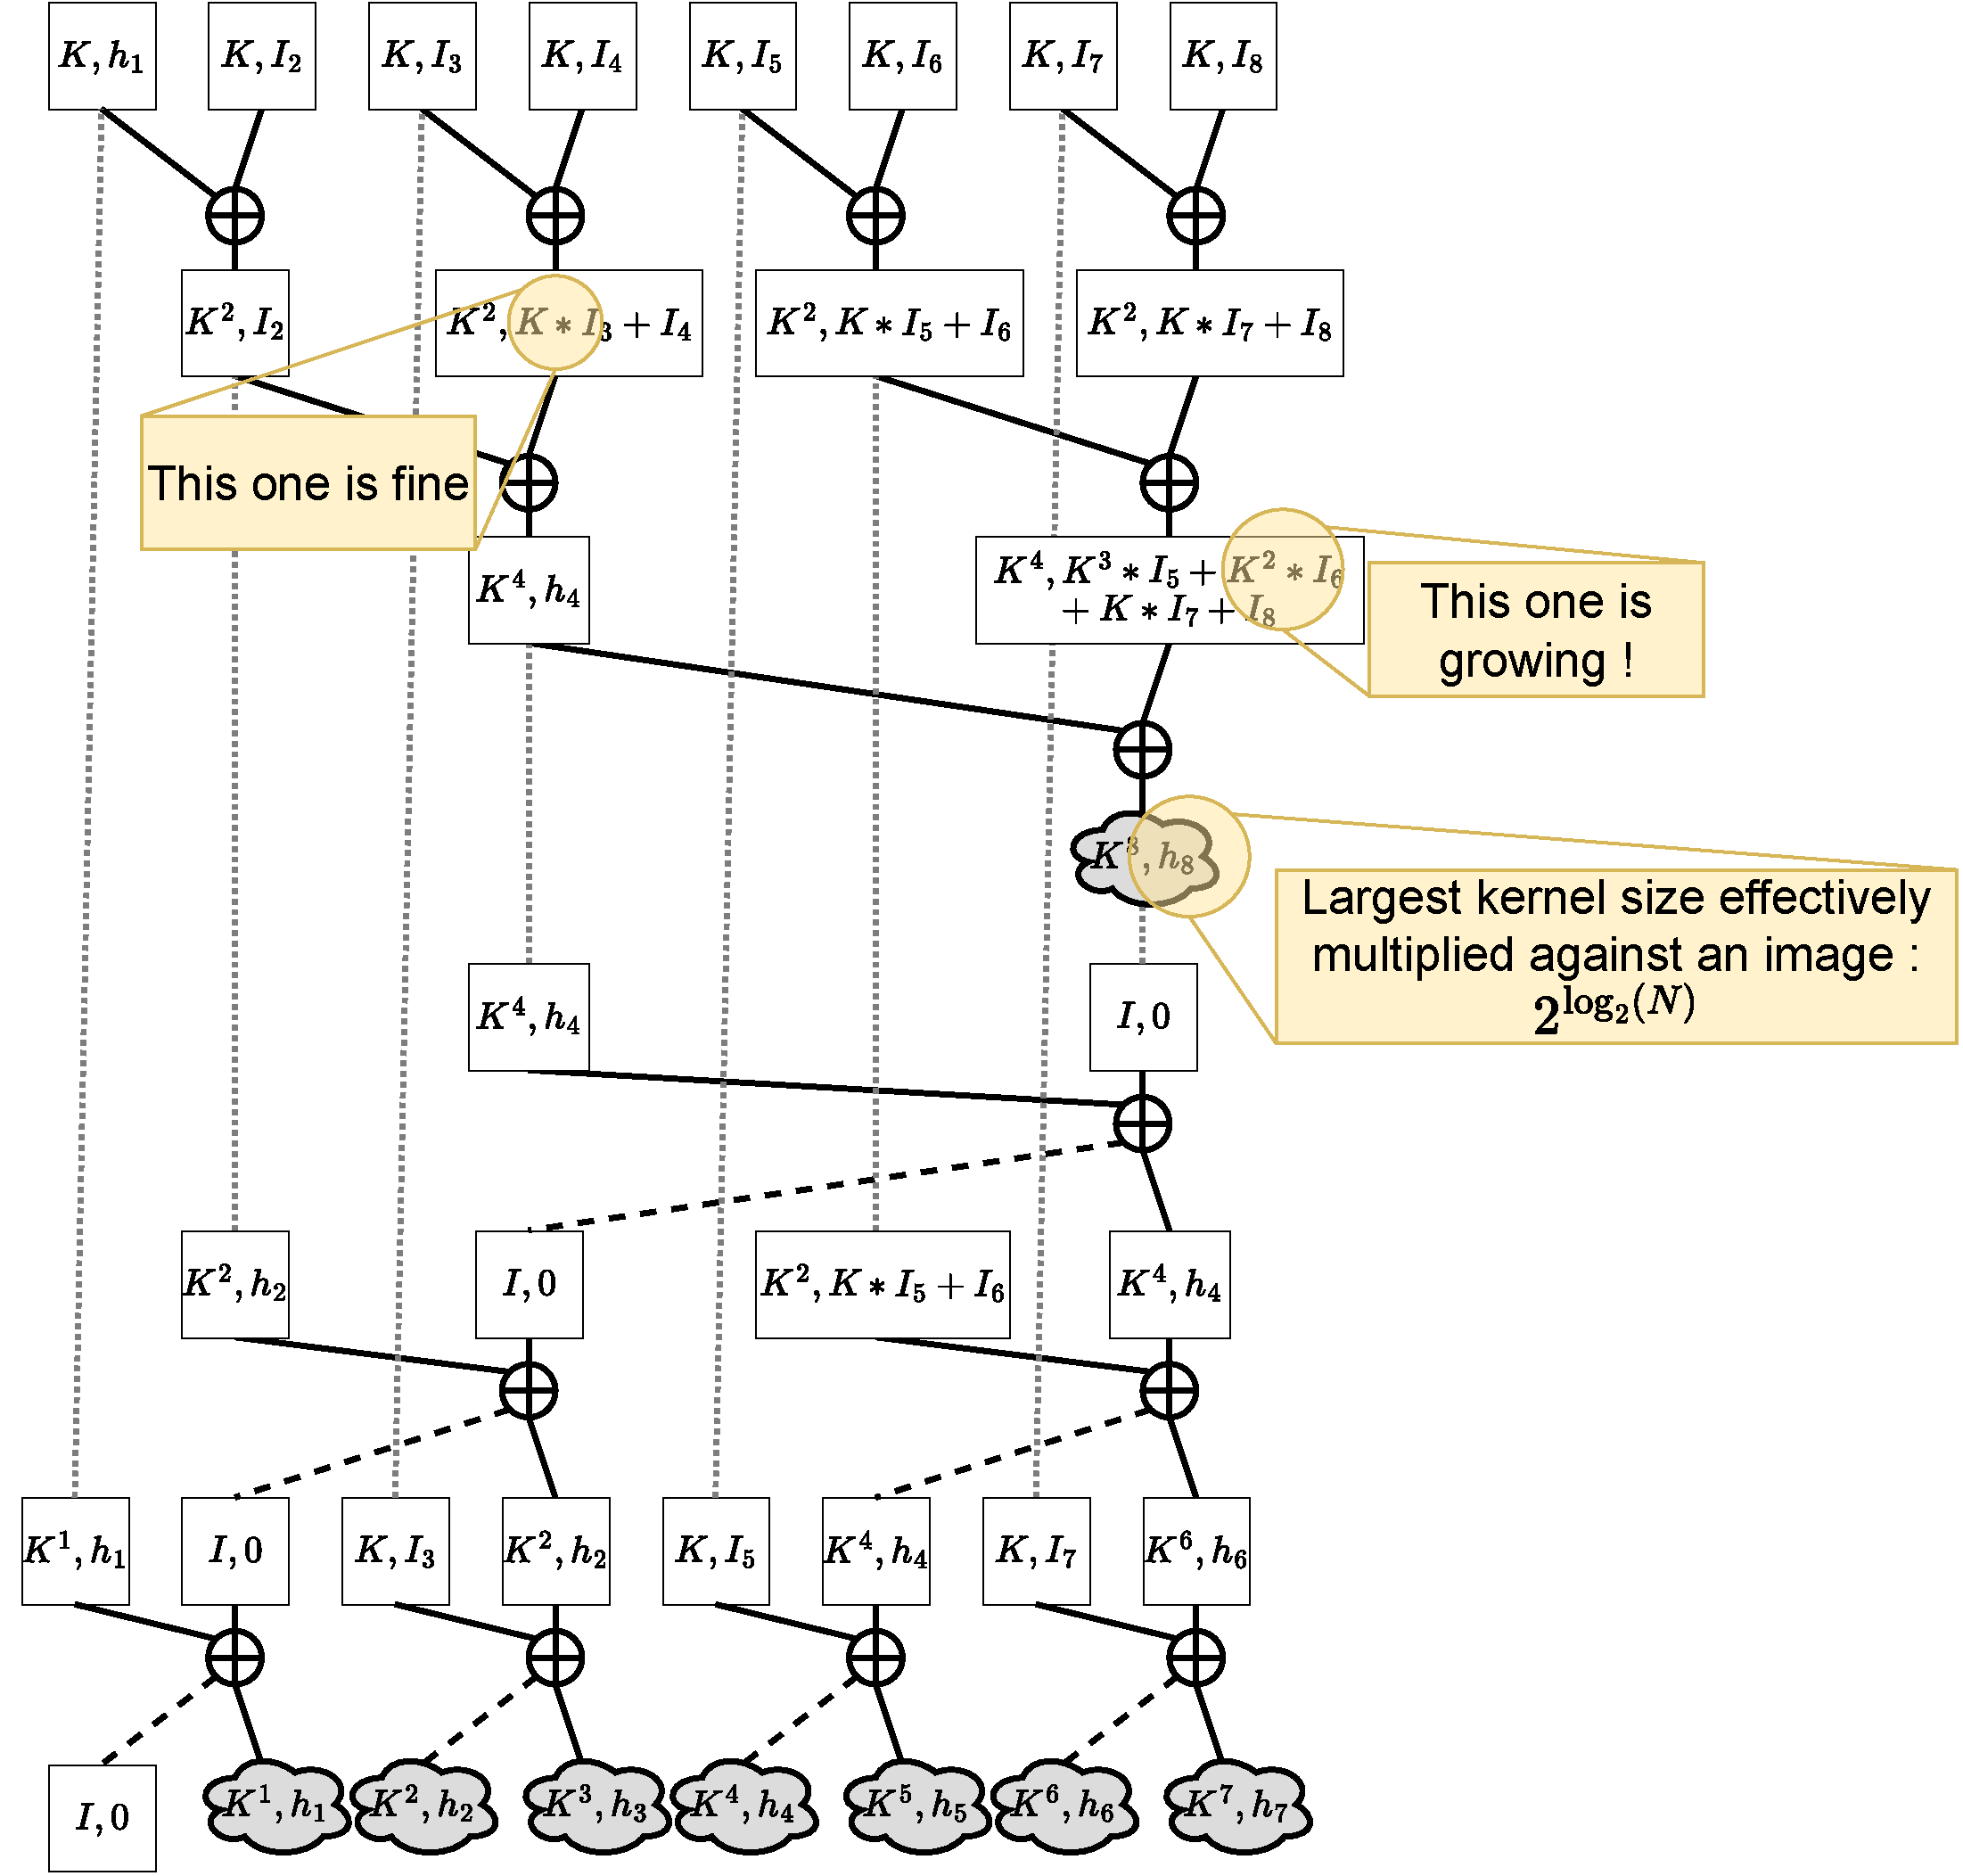
\includegraphics[height=0.3\textheight]{figures/scan_conv.pdf}
    \caption{Parallel scan applied to the monoid structure defined for spatial convolution SSM. Highlighted is the core of the issue : growing kernels lead to a bottleneck where a single operation has $O(T^2)$ complexity.}
    \label{fig:parallel_scan_conv_spatial}
\end{figure}

\subsection{How spectral domain solves the issue}
\label{sec:spectral_ConvSSM}

To dispell the curse of growing kernels we move to the spectral domain. In this domain, our monoid becomes:
\begin{align}
\label{eq:M_SSM_spectral}
    &M^{\mathrm{Conv}_2}\coloneqq \left\{ a = (\hat{K}, \hat{I})\,\middle|\,\exists (K, I)\in M^{\mathrm{Conv}_1},\Bigl\{
\begin{aligned}
    &\hat{K} = \mathrm{FFT}(K_{\mathrm{padded}})\in \C^{h\times w\times c\times c}\\
    &\hat{I} = \mathrm{FFT}(I)\in \C^{h\times w\times c}
\end{aligned}
\Bigr.\right\}\\
\label{eq:+_SSM_spectral}
    &(\hat{K}_a, \hat{I}_a) +^{\mathrm{Conv}_2} (\hat{K}_b,\hat{I}_b)\coloneqq (\hat{K}_b \odot \hat{K}_a, \hat{K}_b \cdot \hat{I}_a + \hat{I}_b)\\
\label{eq:0_SSM_spectral}
    &0\coloneqq(I, 0)
\end{align}
\noindent with $\odot$ the element-wise matrix multiplication and $\cdot$ the element-wise matrix-vector multiplication. With this operator, the kernel grows no more, the cost is again a constant of time and depth, depending only on $h$, $w$ and $c$. We are thus back to a time complexity for the parallel scan of $O(\log T)$.

\begin{proposition}[Spectral ConvSSM Complexity]
\label{prop:spectral_conv_complexity}
    Let $(M, +) \coloneqq (M^{\mathrm{Conv}_2}, +^{\mathrm{Conv}_2})$ be the monoid defined by \Cref{eq:M_SSM_spectral,eq:+_SSM_spectral,eq:0_SSM_spectral}. Let $(a_i)_{i\in I}\in (M^{\mathrm{Conv}_2})^I$.

\begin{align}
    W&= O(T)\\
    T_\infty&= O(\log_2T)
\end{align}
\end{proposition}

\begin{proof}
The proof of \Cref{prop:scan_integer_complexity} applies with the only difference that now, each $+^{\mathrm{Conv}_2}$ operation has complexity $h \times w \times c^3$ for the kernel-kernel multiplication on the left, $h \times w \times c^2$ for the kernel-image multiplication and $h \times w \times c$ for the image addition on the right. This gives :

\begin{align}
\label{eq:W_spectral}
    W&= O(T \times h \times w \times c^3)\\
\label{eq:T_spectral}
    T_\infty&= O(\log_2T \times h \times w \times c^3)
\end{align}
\end{proof}

% \section{Recurrence kernel parameterisation}

% TODO : capability subsection vs complexity subsection vs optimisation subsection

% capability :
% - log domain : multiplicative dynamics in log domain match biological divisive norms. Write it up properly : K*I + I in spatial or spectral is linear, but K*I + I in cepstral becomes K*I * I in spectral - this is the multiplicative dynamic.
% - scale equivariance through wavelets
% - diagoanlisable vs non diagonalisable comment : tradeoff between complexity (cref(sec:TODO below)) and expressivity.
% - anything else ?

% complexity :
% - log domain : This preserves the complexity analysis of section \cref{sec:spectral_ConvSSM}, as you only need to change $+^{\mathrm{Conv}_2}$ such that the right hand side multiplies element wise the images instead of adding them. Then we can operate in log domain.
% - in the fourier space K*K is in $c^3$, and K*I is in $c^2$ (\cref{eq:W_spectral,eq:T_spectral}) : if every frequency bin is diagonalisable, NPLR (normal plus low rank) or something, then this cost can be cut down to $c$ for both. Question : how to actually parameterise spatial domain to have this spectral property ? Would it be easier to parameterise in fourier with constraints such that the spatial domain of the kernel is still k*k ?
% - anything else ?

% optimisation :
% - log domain : It makes BPTT much easier as exponential behaviors mess up gradients but in log domain it is linear
% - orthogonal convolution : this also controls exponential behavior through eigenvalues of 1, but it comes at the cost of expressivity and doesn't have the divisive behavior in log domain. Maybe combine both log domain and orthogonal convolution ? though with log domain you already have what orthogonal brings to the table so maybe it's a bad idea and you just lose expressivity...
% - anything else ?

\subsection{Taking down the constant}
\label{sec:the_constant}

Now that we have solved the main issue of complexity explosion with time, we tackle the problem of the constant. As mentioned in \Cref{prop:SSM_complexity}, as is, the work complexity is $O(T)$ with a constant that is $O(d^3)$ due to matrix multiplications.
\citet{TODO:S4SSM} proposed to reparameterise the recurrence matrix $A$ to be normal plus low rank (NPLR) in order to reduce this constant from $O(d^3)$ to $O(d)$. The complexity gain comes from the change of basis being absorbed outside of the recurrence such that the recurrence can operate on diagonalized matrices. Note that their approach to parallelization through time uses the convolution view of the SSM, not the parallel scan as proposed by \citet{TODO:S5SSM}.
In our case, this $O(c^3)$ is even more prohibitive as it is repeated over each pixel position, with the total constant being $O(k^2c^3 + hwk^2c^2)$ in the spatial domain, and $O(hwc^3)$ in the spectral domain.

In spatial domain, this parameterization translates to having a shared change of basis $V$ for each $K_{x,y}$. This way, $V$ can be factored our ot the kernel such that the resulting kernel follows~: $\forall x,y, \mathcal{K}_{x,y} = \Lambda_{x,y} + P_{x,y} Q_{x,y}^\top$, where
\begin{itemize}
    \item $\Lambda_{x,y}$ are block diagonal with blocks of rank at most $2$ in real domain, and diagonal with eigenvalues of modulus 1 in complex domain. With the complex view, $\mathcal{K}$ is diagonal plus low rank (DPLR).
    \item $P_{x,y}, Q_{x,y} \in \R^{d\times r}$ are low rank matrices, with rank $r$
\end{itemize}
In spectral domain, and after proper zero padding, such a parameterization yields~:

\begin{align*}
    \forall w_1,w_2, \widehat{\mathcal{K}}_{w_1,w_2} &= \sum_{x,y} \alpha_{w_1,w_2}^{x,y} \mathcal{K}_{x,y}\\
    &= \sum_{x,y} \alpha_{w_1,w_2}^{x,y} \left(\Lambda_{x,y} + P_{x,y} Q_{x,y}^\top\right)\\
    &= \sum_{x,y} \alpha_{w_1,w_2}^{x,y} \Lambda_{x,y} + \sum_{x,y} \alpha_{w_1,w_2}^{x,y}P_{x,y} Q_{x,y}^\top\\
\end{align*}

\noindent where $\alpha_{w_1,w_2}^{x,y} = e^{-2\pi i(\frac{w_1x}{h}+\frac{w_2y}{w})}$. There are a couple issues with this~:
\begin{itemize}
    \item The diagonal terms in spatial domain yield diagonal terms in spectral domain. However, these do not have modulus 1, and thus are not stable.
    \item The spectral term coming from the low rank terms is not low rank anymore : it now has rank up to $k^2r$ instead of $r$. This issue can be solved by fixing $P_{x,y}=p,~Q_{x,y}=q$ to be constants. This way, the associated spectral term is low rank.
\end{itemize}
We can circumvent both issues by parameterizing directly in the spectral domain. The tradeoff is that now,
\begin{itemize}
    \item we are bound to a fixed resolution,
    \item the underlying spatial kernel has arbitrary support.
    \item the number of parameters in spectral domain is $hwc(2r+1)$ compared to $k^2c(2r+1)$ in spatial domain.
\end{itemize}
As \citet{TODO:franck} showed that parameterization of CNNs in spectral domain works just fine, we leave the question of finding a parameterization directly in pixel space to future work. Additionally, \citet{TODO} showed that parameterizing the recurrence through a simple normal matrix is as expressive as the NPLR case. We thus take $r=0$ and drop the low rank terms.

% note : mention that \citet{TODO} showed that NPLR parameterisation is no more expressive than normal, in the case of linear SSMs, so in our case we can just remove it.


% ----------------------------------------------------------------------------------------------------
\section{Towards Feedback Connections}
% ----------------------------------------------------------------------------------------------------
\label{sec:ConvSSM_feedback_connections}

\input{sections/part_convssm/feedback_connections.tex}

% ----------------------------------------------------------------------------------------------------
\section{Further Parameterizations}
% ----------------------------------------------------------------------------------------------------

\paragraph{}log domain (GOOM) / multiplicative behavior (might not need log domain if well parameterized, but log domain will help anyway) : circuit : F can include multiplicative or divisive interactions and modulations.

% ----------------------------------------------------------------------------------------------------
Ullman, S. (1984). Visual routines. Cognition, 18(1–3), 97–159. DOI: 10.1016/0010-0277(84)90023-4. 
\section{Experiments}
% ----------------------------------------------------------------------------------------------------

\paragraph{Baselines and SOTA.}SOTA : (h)Gru, ConvS4, ViT, ConvNeXt, etc. baselines : CNN ?

\paragraph{Classification.}imagenet and compagnie

\paragraph{Visual Reasoning.}static : pathfinder, cABC, 3D-PC, planko. Dynamic : feature tracker, pathtracker. Interpretability : attribution vs time, representation alignment, dynamics (attractors, fixed points, etc.), accuracy vs time / accuracy vs convergence to fixed points if any. Graal : pathfinder : have a window of attention moving along the path through time.

\paragraph{Self-Supervised Learning.}dino like ssl, video ssl, predictive coding... interpretability : optical flow, motion prediction, modulation of activation and attribution maps in static areas, representation alignment with other sota ssl models.

% ----------------------------------------------------------------------------------------------------
\section{Scaling Laws}
% ----------------------------------------------------------------------------------------------------

\paragraph{}how does performance scale with model size, data size, compute, etc. ?

% ----------------------------------------------------------------------------------------------------
\section{Foundational ConvSSM}
% ----------------------------------------------------------------------------------------------------

\paragraph{}toy : visual reasoning tasks, generalisation / fine tuning on a held out task.

\paragraph{}large scale : ssl then evaluate on downstream tasks.

% ----------------------------------------------------------------------------------------------------
\section{Quantization}
% ----------------------------------------------------------------------------------------------------

\paragraph{}

% ----------------------------------------------------------------------------------------------------
\section{Discussion}
% ----------------------------------------------------------------------------------------------------

\paragraph{}...

%\part{Interpreting Multimodal Models through the Lens of Neural Circuits} % applying neural circuit interpretability tools to multimodal models, drawing insights and comparisons. (XAI, mech interp, etc.)
% ====================================================================================================
\part{Analyzing Multimodal Models}
% ====================================================================================================

\section*{Part Outline}

\paragraph{}This part is independent on the previous one. It focuses on integrating several unimodal circuits into a single multimodal one. Its goal is not to introduce new architectures, but to analyse existing multimodal models through the lens of neural circuits, using interpretability tools.

% ----------------------------------------------------------------------------------------------------
\section{Related Work}
% ----------------------------------------------------------------------------------------------------

\paragraph{}interpretability, multimodality, etc.

% ----------------------------------------------------------------------------------------------------
\section{The Phenomenology of Multimodal Integration in LMMs}
% ----------------------------------------------------------------------------------------------------

\subsection{Framework Formulation}

\paragraph{}cf je sais plus quel overleaf.

\subsection{Cycle Consistent IsoEnergy SAEs}

\paragraph{}Rewrite $P_{\mathrm{tr}}$, $P_{\mathrm{cont}}$, $P_{\mathrm{dcy}}$, and $P_{\mathrm{cy}}$ from rufin et al., say that $P_{\mathrm{tr}}$ and $P_{\mathrm{cont}}$ rely on patching pairs for translation and alignment, which may not exist, but if the geometry aligns and arise from shared dictionaries, replacing them with IsoEnergy constraints should work. Define $P_{\mathrm{iso}}$ accordingly. Link to dhimoila et al. Show that the method works in a case where we have access to actual cycle consistent losses (e.g. CLIP).

figures : ...

tables : metrics ...

\subsection{Dynamics of Multimodal Integration Across Layers}

\paragraph{}figures : (i) similarity matrices T1(L) vs T2(L'), or similarly with images : T1 is the distribution of text tokens without context, T2 is the distribution of text tokens with image context. If there is significant shift from T1 to T2, it means that image context is integrated into text tokens. (ii) similarity matrices T1(L) vs T1(L') : if significant shift, it means that the model is changing the geometry of the representation space across layers. This should be obvious in T as input tokens are raw and uncontextualised. The interesting case is for I as "input" tokens are already fully refined by the visual system. (iii) similarity matrices T1(L) vs I1(L') : this needs matching pairs or isoenergy constraints to work... enter CCIE SAEs. Expect image and text to get closer across layers maybe until the last few layers where text needs to collapse for token prediction. Under assumption 2 : wasserstein between distributions. Possibly include translation / scale invariance by normalising representations first. Under assumption 3 : SAE based metrics.

\greg{TODO : normalise CMAP in the range of the metric. Currently, plots that range between 0 and 1e-11 will have as bright of a color as plots that have the full range 0-1 or 0-2.}
\greg{have different color maps for different metrics of distribution alignment.}

\begin{figure}[h]
    \centering
    \begin{subfigure}{0.2\linewidth}
        \centering
        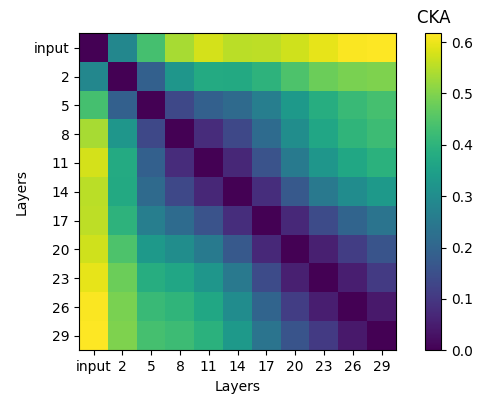
\includegraphics[width=\linewidth]{figures/text_embedding_trajectory_CKA.png}
        \caption{Text distribution}
        \label{fig:phenomenology_text_refinement}
    \end{subfigure}
    \hfill
    \begin{subfigure}{0.2\linewidth}
        \centering
        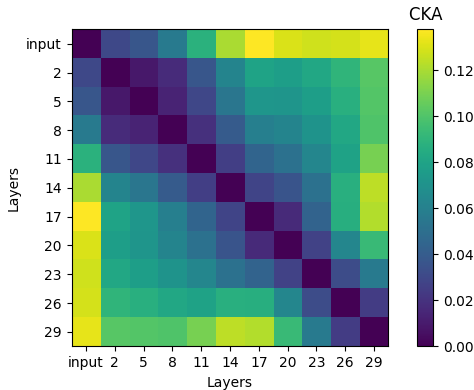
\includegraphics[width=\linewidth]{figures/image_embedding_trajectory_CKA.png}
        \caption{Image distribution}
        \label{fig:phenomenology_image_refinement}
    \end{subfigure}
    \caption{Similarity matrices showing the evolution of text (\emph{left}) and image (\emph{right}) token distributions across layers in a multimodal model. The evolution of text token across layer is standard, and shows that contextualisation and refinment occurs across layers, starting from uncontextualised raw tokens. Visual token evolution is of particular interest here, as visual tokens are already fully refined by the vision backbone. Any significant change in their geometry across layers indicates further refinement or contextualisation performed by the language backbone. \greg{TODO : interpret the actual results.} The metric reported here is \textbf{TODO}. See \cref{sec:...} for other metrics.}
    \label{fig:phenomenology_refinement}
\end{figure}

\begin{figure}[h]
    \centering
    \begin{subfigure}{0.2\linewidth}
        \centering
        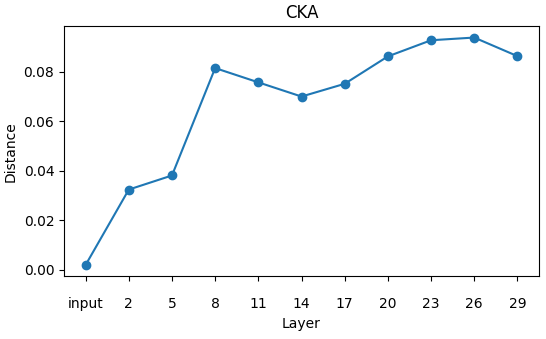
\includegraphics[width=\linewidth]{figures/txt_raw2cond_CKA.png}
        \caption{Text integration}
        \label{fig:phenomenology_text_integration}
    \end{subfigure}
    \hfill
    \begin{subfigure}{0.2\linewidth}
        \centering
        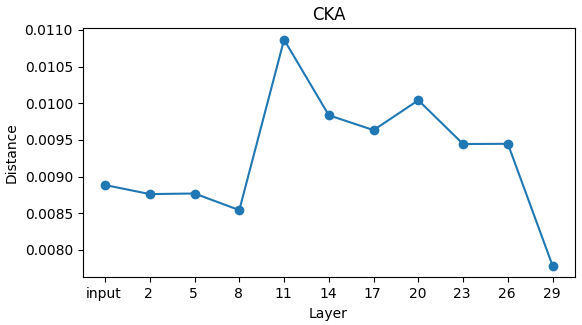
\includegraphics[width=\linewidth]{figures/img_raw2cond_CKA.png}
        \caption{Image integration}
        \label{fig:phenomenology_image_integration}
    \end{subfigure}
    \caption{Multimodal integration dynamics across layers. Contrary to \cref{fig:phenomenology_refinement}, which focused on the evolution of the geometry of each modality independently, here we focus on the effect of multimodal integration on this geometry. Specifically, we compare the distribution of text tokens without image context to the distribution of text tokens with image context (\emph{left}), and similarly for image tokens (\emph{right}). The diagonal of this distance matrices is of particular interest, as the off diagonal elements are mainly driven by layer-wise drift of the geometry rather than multimodal integration effects. \greg{TODO : interpret the actual results.}}
    \label{fig:phenomenology_integration}
\end{figure}

\begin{figure}[h]
    \centering
    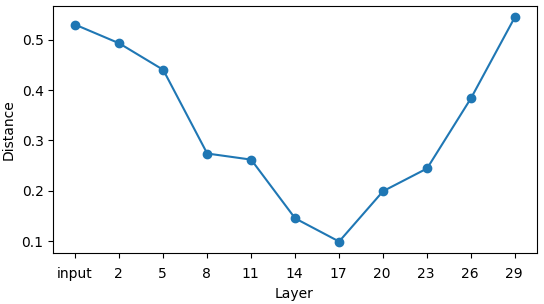
\includegraphics[width=0.2\linewidth]{figures/img2txt_Wasserstein.png}
    \caption{Geometric similarity between text and image token distributions across layers. This figure shows how the geometry of text and image token distributions align across layers in a multimodal model. \greg{TODO : interpret the actual results. Both distributions seem to converge to a shared latent geometry. If the previous figures shows that image geometry is roughly constant, we should see stripes of equal alignment}}
    \label{fig:phenomenology_text_integration}
\end{figure}

% ----------------------------------------------------------------------------------------------------
\section{Interpretability of Multimodal Integration in LMMs}
% ----------------------------------------------------------------------------------------------------

\subsection{Identifying Multimodal Neurons}

\paragraph{}e.g. a "blue" neuron that responds to both the concept of "blue" in text and images. Use SAEs for automated identification, e.g. the whole Gamma subspace if that works, or probes for specific concepts. causal intervention : fiddle with these neurons and check for predictable effect on both vision and language token fiddling.

\subsection{Visual Integration Circuits}

\paragraph{}Are there dedicated circuits that move information from vision tokens to language tokens ? Or does the visual token just align with latent geometry and the information retrieval follows arbitrary pre existing language circuits ? Start with task specific then move on to general ones. causal interventions : 1st case : ablate these circuits, check that text only capabilities are preserved but vision integration is lost. 2nd case : since these are not dedicated multimodal integration pathways but recycled unimodal language circuits leveraged through representational alignment, ablating them should break both vision integration and text only capabilities. This gives two hypotheses that can be tested experimentally.

\subsection{On the Binding Problem}

\paragraph{}there might not be a binding problem at all... in LMM, it's either trivially solved when there is no more than one object of interest per token, or unsolved due to the vision backbone, not due to multimodal integration per se.

% ----------------------------------------------------------------------------------------------------
\section{Discussion}
% ----------------------------------------------------------------------------------------------------

\paragraph{}...

% ====================================================================================================
\part{Towards Multimodal Neural Circuits} % proposing new multimodal architectures inspired by neural circuits, integrating insights from previous parts. If time permits implementation and experiments, include interpretability analysis based on the previous part.
% ====================================================================================================

\section*{Part Outline}

\paragraph{}Combining insights from parts II and III, we propose new multimodal architectures inspired by neural circuits in light of what we learned. (speculative part for now)

% ----------------------------------------------------------------------------------------------------
\section{Introduction}
% ----------------------------------------------------------------------------------------------------

\paragraph{}multimodal, embodied agents, neural circuits, patati patata...

% ----------------------------------------------------------------------------------------------------
\section{Related Work}
% ----------------------------------------------------------------------------------------------------

\paragraph{}...

% ----------------------------------------------------------------------------------------------------
\section{...}
% ----------------------------------------------------------------------------------------------------

\paragraph{}...

% embodied agents & co, make an architecture with sensory and motor circuits that all interact, cooperate and condition each other.

% ====================================================================================================
\part{Universal Neural Circuits} % similar to universal turing machines, propose a universal machines that takes as input a history of h_{W \subseteq V}(t) over time and predicts the next states h(T+k)
% ====================================================================================================
% modivation sEEG dataset, build a foundation model for brain science.
% Plan :
% - theoretical framework, results and analysis. Find out under which hypotheses universal circuits can exist, find bounds for zero or first order approximation, etc...
% - foundational UNC architecture
% - finetune on brain data
% - finetune on sEEG data

\section*{Part Outline}

\paragraph{}We propose the notion of universal neural circuits (UNC), akin to universal turing machines, that can simulate any other neural circuit under some constraints. This could serve as a foundation model for brain science.

% ----------------------------------------------------------------------------------------------------
\section{Introduction}
% ----------------------------------------------------------------------------------------------------

\paragraph{}EEG, MEG, sEEG, etc. Foundation models for brain science.

% ----------------------------------------------------------------------------------------------------
\section{Related Work}
% ----------------------------------------------------------------------------------------------------

\paragraph{}...

% ----------------------------------------------------------------------------------------------------
\section{...}
% ----------------------------------------------------------------------------------------------------

\paragraph{}...

% ====================================================================================================
\part{Appendix} % Start the appendix part
\parttoc % Insert the appendix TOC

\section{State Space Models.}
\label{sec:SSM}

\paragraph{} 
Neural circuits rely heavilly on recurrent connections, key to model long range dependencies and working memory. However, training recurrent neural networks is notoriously difficult due to vanishing and exploding gradients on the optimisation side, and to sequentiality incompatible with modern hardware acceleration on the computational side. Recently, state space models (SSMs) have emerged as a powerful class of models to tackle these issues. The core idea of SSMs is to model the recurrent dynamics as a linear system, allowing to leverage linear algebra tools to parallelise training and inference, while maintaining the ability to model long range dependencies through carefully designed dynamics. See \cref{sec:ConvSSM_definition} for a formal definition and analysis of the stability of these systems. See \cref{sec:ConvSSM_complexity} for a detailed analysis of their computational complexity in light of modern hardware acceleration.
%
SSMs have been successfully applied to various domains, including natural language processing \citep{TODO}, computer vision \citep{TODO}, and time series analysis \citep{TODO}.

\end{document}
